% Første linje er dokumentklassen. Brug *altid* memoir!
\documentclass[a4paper,oneside,article]{memoir}

% Herunder indlæses forskellige pakker
\usepackage[utf8]{inputenc}  % Korrekt håndtering af æ, ø og å
\usepackage[T1]{fontenc}  % Korrekt håndtering af æ, ø og å
\usepackage{microtype}  % Typografisk magi! Giver bl.a. pænere orddeling
\usepackage{graphicx}  % Gør det muligt at indsætte billeder
\usepackage{amsmath, amssymb}  % Giver adgang til uundværlige matematikting
\usepackage{mathtools}  % Retter ting i ams og giver ekstra muligheder
\usepackage[danish]{babel}  % Danske betegnelser og orddeling
\usepackage{lmodern}
\usepackage{alphabeta}
\usepackage{float} %Mere kontrol over billede-placering
\renewcommand{\danishhyphenmins}{22}  % Bedre dansk orddeling
\usepackage[exponent-product=\ensuremath{\cdot}]{siunitx} % Sientific notation for forskellige ting, med en regel om at den skal bruge cdot istedet for times. 
\usepackage{derivative} % Til at skrive differentialligninger 
\usepackage{xcolor} % For at få flere tekst farver 
\usepackage[colorlinks=true]{hyperref} % For at få refrences man kan trykke på, slet [] hvis man vil have kasser i stedet for farvet tekst.
\usepackage{pdfpages} % Til at indsætte andre pdf'er
\usepackage{subfig} % For at have to billeder ved siden af hinanden
\usepackage{unicode-math}
\usepackage{bm}
\usepackage{tabularx}

\usepackage{listings}
% Global settings for listings
\lstset{
  basicstyle=\ttfamily\footnotesize,
  keywordstyle=\color{blue},
  commentstyle=\color{green!60!black},
  stringstyle=\color{purple},
  numbers=left,
  numberstyle=\tiny\color{gray},
  breaklines=true,
  captionpos=b,
  % For inline:
  literate=*{:}{{\textcolor{red}:}}1 {=}{{\textcolor{red}=}}1 {()}{{\textcolor{blue}()}}2, % Example to color specific characters
}



% Pænere toc indents 
\usepackage{tocloft}
\cftsetindents{section}{1em}{2em}
\cftsetindents{subsection}{4em}{0em}


% Indholdet i dit dokument starter her!
\begin{document}

%Custom Commands
%Til opgavebeskrivelser
\newcommand{\opg}[1]{\textcolor{gray}{\emph{#1}}\plainbreak{1}} 

\newcommand{\ti}[1]{\cdot 10^{#1}} % Let: gange 10^x
\newcommand{\e}[1]{\emph{e}^{#1}} % Pænere e^x
\newcommand{\vm}[2]{\begin{pmatrix} #1 \\ #2 \end{pmatrix}}
\newcommand{\mat}[1]{\begin{bmatrix} #1 \end{bmatrix}}
\renewcommand{\v}[1]{\mathbfit{#1}}

% Lette paranteser 
\newcommand{\br}[2][1]{%
\ifcase#1
\or \left( #2 \right) %1 eller ingenting
\or \left[ #2 \right] %2
\or \left\langle #2 \right\rangle %3
\or \left\{ #2 \right\} %4
\or \left| #2 \right| %5
\fi
}
%Til at sætter bileder ind i store dokumenter
\newcommand{\bil}[1]{
    \begin{figure}[H]
        \centering
        \includegraphics[width=0.75\linewidth]{Billeder/#1.png}
        \label{fig:#1}
    \end{figure}
    }
    
%Til at sætte pdf'er ind i store dokumenter (kun pdf'er på mere end 1 sider)
\newcommand{\pdf}[4]{
    \includepdf[pages=#3,scale=.85,pagecommand={\subsection{#2 - \ref{ch:opg}}  \label{asc:#2}}]{pdf/#1.pdf}
    \includepdf[pages=\the\numexpr 1 + #3\relax-#4, scale=.85]{pdf/#1.pdf}
}

\newcommand{\h}{\hbar}
\newcommand{\dd}{\partial}
\newcommand{\eq}[1]{\label{eq:#1}\tag{#1}}
\renewcommand{\a}{\hat{\v{a}}}
\newcommand{\n}{\plainbreak{1}}
\newcommand{\ep}{\epsilon_0}
\renewcommand{\r}{\text{\usefont{U}{dutchcal}{m}{n}r}}
\newcommand{\elcon}{\frac{1}{4π\ep}}
\newcommand{\emf}{\mathscr{E}}

\newcommand{\hv}[2][]{%
    \if\relax\detokenize{#1}\relax
        |#2\rangle%
    \else
        \if\relax\detokenize{#2}\relax
            \langle #1|%
        \else
            \langle #1|#2\rangle%
        \fi
    \fi
}


\newcommand{\code}[1]{\lstinline|#1|}
 
 
% Lav ny pagestyle (kun odd fordi enkeltsidet)
\makepagestyle{Title}
\pagestyle{Title}
%\makeoddhead{Title}{\footnotesize\color{gray}{\theauthor}}{}{\textcolor{gray}{\thedate}}
\makeoddfoot{Title}{}{\footnotesize\color{gray}{\thepage{} / \thelastpage}}{}
% Også fod på siden med \maketitle
\makeoddfoot{plain}{}{\footnotesize\color{gray}{\thepage{} / \thelastpage}}{}
\newpage
 
%Skriv
%%%%%%%%%%%%%%%%%%%%%%%%%%%%%%%%%%%%%%%%%%%%%%%%%%%%%%%%%%%%%%%%%%%%%%
%% Front page
%%%%%%%%%%%%%%%%%%%%%%%%%%%%%%%%%%%%%%%%%%%%%%%%%%%%%%%%%%%%%%%%%%%%%%

\thispagestyle{empty}
\setcounter{page}{0}

\begin{center}
  \huge
  \textbf{Introduction to Programming \\
  with Scientific Applications \\
  (Spring 2025)} \\[2ex]
  Final project \\[3ex]
\end{center}
\noindent
\begin{tabularx}{\textwidth}{|c|X|c|}
\multicolumn{1}{c}{Study ID} & 
\multicolumn{1}{l}{Name} & 
\multicolumn{1}{l}{\% contributed} \\
\hline
202307989 & Mikkel Moth Billing & 100\% \\ % Student 1
\hline
& & \\ % Student 2
\hline
& & \\ % Student 3
\hline
\end{tabularx}
\centerline{max 3 students}
\\[2ex]
\noindent
Briefly state the contributions of each of the group members to the project
\\
\begin{tabularx}{\textwidth}{|X|}
\hline
% Your comment goes here
I did all the coding and the report writing.  
\\[2ex]
\hline 
\end{tabularx}
\\[2ex]
\noindent
Declaration on Generative Artificial Intelligence (see \url{https://studerende.au.dk/en/gai})
\\
\begin{tabularx}{\textwidth}{|X|}
\hline
% Your comment goes here
\textbf{I used generative artificial intelligence (GAI) to complete this project. }
I used ChatGPT and Copilot to help with bugfixing and to get a better understanding of the processes of machine learning. 

I have stated what i have used GAI for in the report. I have not coppied code just used it for inspiration. 
\\[3cm]
\hline 
\end{tabularx}


\vfill
\noindent
\textbf{Note on plagiarism} 
\\[2ex]
Since the evaluation of the project report and code will be part of the final grade in the course, \textbf{plagiarism in your project handin will be considered cheating at the exam}. Whenever adopting code or text from elsewhere you must state this and give a reference/link to your source. It is perfectly fine to search information and adopt partial solutions from the internet -- actually, this is encouraged -- but always state your source in your handin. Also discussing your problems with your project with other students is perfectly fine, but remember each group should handin their own solution. If you are in doubt if you solution will be very similar to another group because you discussed the details, please put a remark that you have discussed your solution with other groups. For more Aarhus University information on plagiarism, please visit \url{http://library.au.dk/en/students/plagiarism/}.

\newpage

%%%%%%%%%%%%%%%%%%%%%%%%%%%%%%%%%%%%%%%%%%%%%%%%%%%%%%%%%%%%%%%%%%%%%%

% Your report text goes here
\chapter{Introduction }
For this project I had to look at Image Classification, by creating a simple neural network. 
This neural network is used to classify images of handwritten difgits from the MNIST database. 
These images are given in 28x28 grayscale images, where each pixel is a number between 0 and 255. 
I then use linear classification using a 784x10 matrix and a bias vector of size 10, to guess the number. 
From this guess we can calulate a cost, which is the mean square error of the guess and the actual number.
By minimizing this cost function using linear algebra, we can update the weght matrix and bias vector. 
The weights can then be visualized and the cost and accuracy can be plotted, to show how the neural network evolves. 

\chapter{Code}
Thoughout the code i have used the decorator \code{@time_it}, that we have from the lectures, to time the functions used. 
\section{Reading Data}
For getting the raw data out of the MNIST files I had to first understand the format of the .gz files. 
For this I have used ChatGPT to help me understand  how to read the bytes in the file, to get the magic numbers. 
Then as we can see at \url{https://github.com/sunsided/mnist} the first 4 bytes of the files are the magic number, 
which is $2049$ for label files and $2051$ for images files. 
Then the files contains 4 bytes decriping the size of the file, additionally the image files contains 8 bytes for the size the images. 
After that we can read the raw data. 

To read the bytes I open the files with \code{gzip.open} then read the files with \code{.read}. 
Then we can plot the images with their correct label, to see that we have read the data correctly, since the first 5 numbers of 
\code{t10k-labels.idx1-ubyte.gz} are \code{[7, 2, 1, 0, 4]} as seen in figure \ref{fig:im1}. 

\begin{figure}[H]
    \centering
    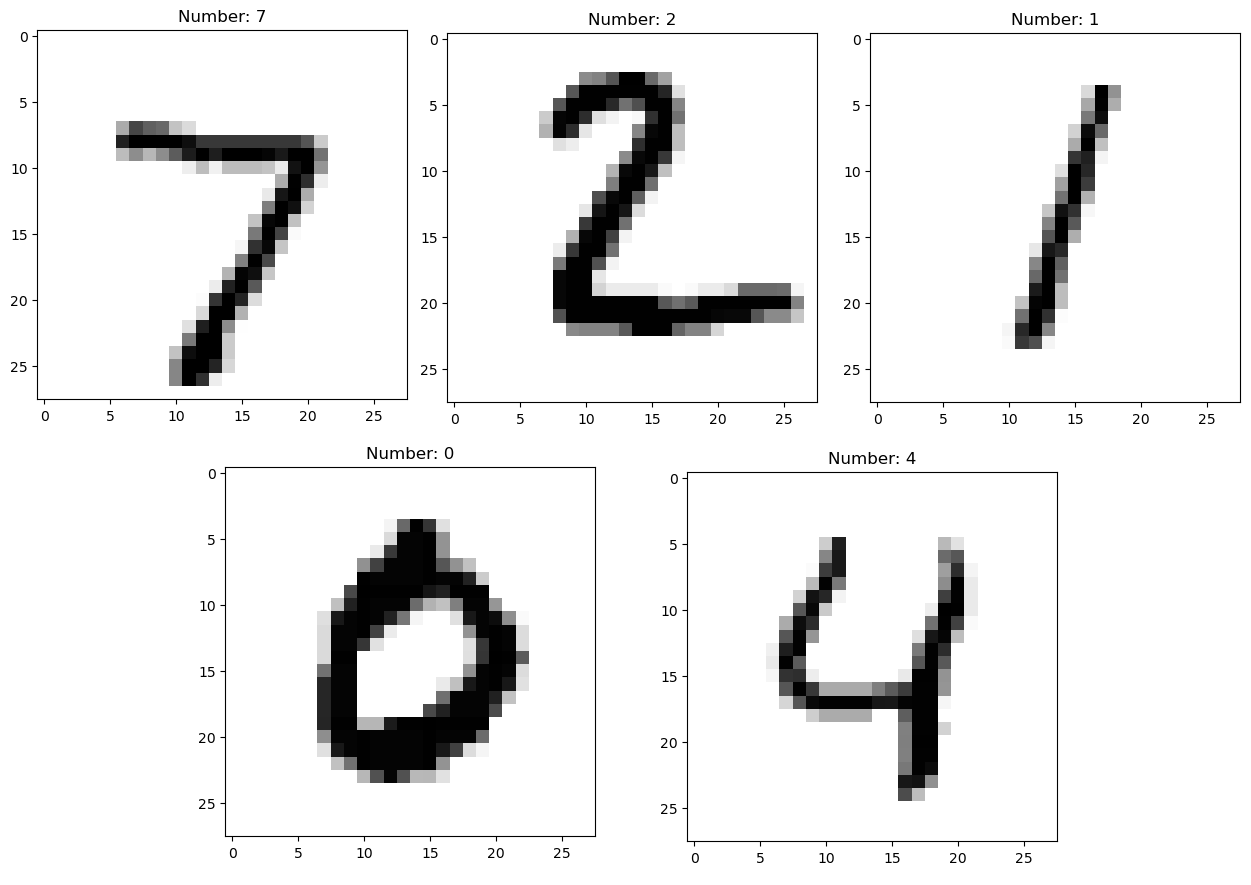
\includegraphics[width=0.55\linewidth]{Billeder/im1.png}
    \caption{The first 5 images of the MNIST test set.}
    \label{fig:im1}
\end{figure}

I also coded a way to read and write JSON files so that the weight matrix and bias vector can be saved. 
This is done with the json library. By doing this we can visualize the weights and biases from MNIST as seen in figure \ref{fig:MNIST}.
\begin{figure}[H]
    \centering
    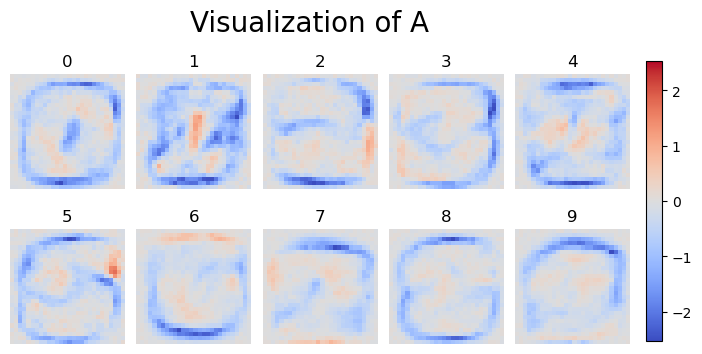
\includegraphics[width=0.7\linewidth]{Billeder/MNIST.png}
    \caption{The weights of the MNIST neural network.}
    \label{fig:MNIST}
\end{figure}

\section{Linear Algebra}
Since numpy is not allowed in the project, I had to write linear algebra functions to use on list vectors and matrices.
These include vector addition, subtraction, and scalar multplication. For these I wrote assertation tests to check if the given vectors are the same length, and that the scalar is actually a number. 

\end{document}